\documentclass[10pt]{article}

\usepackage{neurips_2026}

\usepackage{amsmath,amssymb}
\usepackage{booktabs}
\usepackage{multirow}
\usepackage{xcolor}
\usepackage{graphicx}
\usepackage{hyperref}
\usepackage{url}
\usepackage{microtype}
\usepackage{natbib}
\usepackage{tikz}
\usepackage{placeins}
\usetikzlibrary{positioning}

\graphicspath{{../figures/}{figures/}}

%% Metric shorthands
\newcommand{\mirror}{\textsc{Mirror}}
\newcommand{\MCI}{MCI}
\newcommand{\CCE}{CCE}
\newcommand{\ARS}{ARS}
\newcommand{\KDI}{KDI}
\newcommand{\CFR}{CFR}
\newcommand{\UDR}{UDR}
\newcommand{\SSR}{SSR}
\newcommand{\FDR}{FDR}
\newcommand{\TII}{TII}
\newcommand{\SAR}{SAR}
\newcommand{\AI}{AI}
\newcommand{\eg}{\textit{e.g.}}
\newcommand{\ie}{\textit{i.e.}}

\title{\mirror{}: A Hierarchical Benchmark for Metacognitive Calibration\\in Large Language Models}

\author{
  Anonymous Authors \\
  NeurIPS 2026 Datasets and Benchmarks Track
}

\setlength{\textfloatsep}{6pt plus 2pt minus 4pt}
\date{}

\begin{document}
\maketitle

% =============================================================================
\begin{abstract}
% =============================================================================
We introduce \mirror{} (Metacognitive Integrity and Recursive Reasoning in
Operationalized Response), a benchmark comprising eight experiments across four
metacognitive levels that evaluates whether large language models can use
self-knowledge to make better decisions. We evaluate 16 models from 8 labs across
approximately 250,000 evaluation instances using five independent behavioral
measurement channels. We find two phenomena with direct implications for agentic
deployment: (1)~compositional self-prediction fails universally---the Compositional
Calibration Error ranges from 0.500 to 0.943 across 15 models, and the
Metacognitive Convergence Index is 0.000, and (2)~models
possess accurate domain-specific self-knowledge but systematically fail to translate
it into appropriate agentic action-selection---external metacognitive control reduces
the Confident Failure Rate from 0.562 to 0.214, a 62\% reduction. Providing models
with their own calibration scores produces no significant improvement ($p > 0.05$);
only architectural constraint is effective. These findings challenge the assumption
underlying current agentic architectures that accurate self-knowledge enables
self-correction, and suggest that external metacognitive scaffolding---not improved
self-knowledge---is the path to safer autonomous AI systems. \mirror{} and all data
are publicly available.
\end{abstract}

% =============================================================================
\section{Introduction}
\label{sec:intro}
% =============================================================================

The deployment of large language models (LLMs) as autonomous agents presupposes a
form of metacognitive competence: the model must not only know \textit{what} it
knows, but must translate that awareness into appropriate action---proceeding when
confident, escalating to tools or human review when uncertain. This assumption
underlies agentic architectures built on self-reflection loops, confidence-based
routing, and Constitutional AI self-monitoring~\citep{perez2022sycophancy}. It is
foundational to the enterprise of agentic AI safety. It has never been
systematically tested.

Prior work has studied LLM calibration~\citep{kadavath2022language,
kapoor2024calibration}, uncertainty estimation~\citep{lin2024generating}, and
situational awareness~\citep{laine2024me}. But these address different questions:
calibration measures whether confidence matches accuracy; situational awareness
measures whether models know \textit{what they are}. Nobody has systematically
tested whether models can \textit{use} their self-knowledge to make better
decisions---whether the bridge from metacognitive \textit{monitoring} to
metacognitive \textit{control}~\citep{nelson1990metamemory} is intact.

We introduce \mirror{}, a hierarchical benchmark spanning four metacognitive levels
(atomic self-knowledge, cross-domain transfer, compositional prediction, and
adaptive self-regulation), eight experiments, and five independent behavioral
measurement channels. We evaluate 16 models from 8 labs across approximately
250,000 evaluation instances.\footnote{Computed as: Exp1 (5,000 $\times$ 5 channels $\times$ 16 models) + Exp4 (320 $\times$ 2 conditions $\times$ 15 models) + Exp9 (597 $\times$ 4 conditions $\times$ 3 paradigms $\times$ 10 models) + Experiments 2, 3, 5, 6, 8 ($\sim$30,000 total). See Section~\ref{sec:benchmark} for per-experiment details.}

Three findings emerge. First, compositional self-prediction fails universally: the Compositional Calibration Error (\CCE{}) ranges from 0.500 to 0.943 across
15 models, and the Metacognitive Convergence Index (\MCI{}) is 0.000---models
that calibrate accurately in individual domains completely fail to
compose those calibrations for multi-domain tasks. Second, the knowing-doing gap:
models possess accurate self-knowledge but do not act on it. External constraint
reduces the Confident Failure Rate (\CFR{}) from 0.562 to 0.214 (62\% reduction);
providing models with their own calibration scores produces no significant
improvement. Third, self-knowledge is domain-atomic: the Transfer Influence Index
ranges from 0.019 to 0.175 across 11 models, indicating that calibration does not
meaningfully cross domain boundaries.

\paragraph{Contributions.}
\begin{itemize}
  \setlength\itemsep{2pt}
  \item The \mirror{} benchmark: 8 experiments across 4 metacognitive levels, 5
        behavioral channels, 5,000 domain-stratified questions, and 597 composite
        agentic tasks, publicly released with all protocols and analysis code.
  \item Two empirical findings---universal compositional failure
        (\MCI{}~=~0.000) and the knowing-doing gap (62\% \CFR{} reduction
        under external control)---that challenge assumptions about LLM
        self-knowledge.
  \item Quantification of the knowing-doing gap's cost: in a 1,000-task agentic
        deployment, $\sim$562 tasks fail silently without external constraint
        versus $\sim$214 with constraint.
  \item Evidence that external metacognitive scaffolding, not better
        self-knowledge, is the path to safer agentic systems.
\end{itemize}

Table~\ref{tab:comparison} positions \mirror{} relative to prior work.

\begin{table*}[t]
\centering
\caption{Comparison of MIRROR with prior benchmarks for LLM self-knowledge and metacognition.}
\label{tab:comparison}
\resizebox{\textwidth}{!}{%
\begin{tabular}{l c c c c c}
\toprule
\textbf{Feature} & \textbf{SAD} & \textbf{Barkan et al.} & \textbf{Kadavath et al.} & \textbf{Steyvers et al.} & \textbf{MIRROR} \\
& \textbf{(Laine 2024)} & \textbf{(2025)} & \textbf{(2022)} & \textbf{(2025)} & \textbf{(Ours)} \\
\midrule
Venue & NeurIPS D\&B '24 & NeurIPS WS '25 & arXiv & arXiv & NeurIPS E\&D '26 \\
Focus & Situational & Self-capability & Calibration & Metacognition + & Metacognitive cal. \\
 & awareness & prediction & (P(IK)) & uncertainty & $\rightarrow$ agentic action \\
Models & 16 & $\sim$15 & $\sim$10 & 2 families & 16 \\
Task categories & 7 & 3 & --- & 6 datasets & 8 experiments \\
Total items & 13K questions & $\sim$1K tasks & --- & 12K+ items & 5{,}597 tasks$^\dagger$ \\
Metacognitive levels & 1 (awareness) & 1 (confidence) & 1 (calibration) & 1 (calibration) & 4 (L0--L3) \\
Behavioral channels & 1 (MC/free) & 1 (verbal) & 1 (verbal) & 1 (verbal) & 5 (wager, opt-out, \\
 &  &  &  &  & tool, diff., natural) \\
Agentic connection & No & Yes (SWE-bench) & No & No & Yes (4 cond., 3 par.) \\
Headline finding & Partial sit. & LLMs over- & \emph{Mostly} & Task-specific & Knowing-doing gap \\
 & awareness & confident & calibrated & metacognition & (62\% CFR reduction) \\
Public dataset & Yes & No & No & No & Yes \\
\bottomrule
\end{tabular}}\\[4pt]
{\footnotesize $\dagger$5,000 domain questions + 597 agentic tasks. Evaluated across 16 models, 5 channels, and multiple conditions, yielding $\sim$250K total evaluation instances.}
\end{table*}

% =============================================================================
\section{Related Work}
\label{sec:related}
% =============================================================================

\textbf{LLM Calibration.}
\citet{kadavath2022language} showed that LLMs can predict their own answer
correctness above chance on knowledge-intensive tasks.
\citet{kapoor2024calibration} demonstrated that fine-tuning is needed for reliable
calibration. \citet{steyvers2025calibration} found that metacognitive ability is
task-specific, not general---a finding consistent with \mirror{}'s domain-level
analysis. \mirror{} differs from all prior calibration work in testing whether
calibration \textit{transfers to action-selection}: we measure the gap between
knowing and doing, not the accuracy of knowing alone.

\textbf{LLM Self-Knowledge and Situational Awareness.}
SAD~\citep{laine2024me} measures whether LLMs know what they are---identity,
lifecycle stage, deployment context. \citet{barkan2025llms} tested capability
prediction on SWE-bench tasks, finding systematic overconfidence.
\citet{xiong2023can} found that LLMs are often overconfident when expressing
numerical probability estimates. \mirror{} is complementary: SAD diagnoses
awareness; \mirror{} diagnoses the gap between awareness and behavior.

\textbf{Agentic Evaluation.}
AgentBench~\citep{liu2023agentbench}, OSWorld~\citep{xie2024osworld}, and
GAIA~\citep{mialon2023gaia} measure task success rate in agentic settings. These
benchmarks evaluate execution quality conditional on the decision to act.
Concurrent work on agentic confidence calibration~\citep{htc2026} measures
calibration during multi-step trajectories using trajectory-level features.
\mirror{} differs in measuring metacognitive calibration \textit{before} deployment
and testing whether pre-deployment assessment predicts agentic outcomes. More
broadly, \mirror{} inverts the standard framing: we measure the \textit{decision}
itself, treating task execution quality as a downstream variable and
calibration-informed decision-making as the primary outcome.
Self-correction approaches---including Reflexion~\citep{shinn2023reflexion},
SelfCheckGPT~\citep{manakul2023selfcheckgpt}, and
chain-of-verification~\citep{dhuliawala2023chainofverification}---test whether
iterative self-reflection improves task performance. \mirror{}'s Experiment~9
tests a complementary question: whether pre-measured metacognitive profiles predict
when self-correction will fail. Selective classification
methods~\citep{geifman2017selective} provide formal frameworks for deciding when
to defer; \mirror{}'s escalation curve evaluates domain-informed selective
classification in agentic settings.
Recent work on explicit safety scaffolding~\citep{mosaic2026} demonstrates that
externalized check-and-refuse loops outperform implicit reasoning for
safety-critical decisions, aligning with \mirror{}'s finding that architectural
constraint outperforms self-knowledge exposure.

\textbf{Metacognition in AI.}
Metacognitive prompting~\citep{wang2024metacognitive} uses metacognitive strategies
to improve LLM performance. Augmented language model surveys~\citep{mialon2023augmented}
document the tool-use landscape but do not address when tool use \textit{should}
occur. Concurrent work on metacognition in large reasoning
models~\citep{metacog2026} tests difficulty awareness, confidence adjustment, and
strategy revision across reasoning models. \mirror{} extends this by connecting
metacognitive assessment to agentic deployment through the Experiment~9 escalation
design, providing the first benchmark-scale empirical test linking metacognitive
assessment to agentic deployment outcomes.

% =============================================================================
\section{The \mirror{} Benchmark}
\label{sec:benchmark}
% =============================================================================

\mirror{} decomposes LLM metacognition into four levels of increasing cognitive
complexity, inspired by the hierarchical structure of human metacognitive monitoring
and control~\citep{flavell1979metacognition, nelson1990metamemory}. At each level,
we measure behavior through five independent channels to prevent format-specific
gaming.

\subsection{Metacognitive Levels}

\textbf{Level 0---Atomic Self-Knowledge (Calibration).}
Can the model accurately estimate $P(\text{correct})$ for a given question in a
given domain? This is the best-studied level~\citep{kadavath2022language,
kapoor2024calibration} and serves as \mirror{}'s foundation. Experiment~1
establishes per-model, per-domain calibration profiles across 8 cognitive domains.

\textbf{Level 1---Cross-Domain Transfer.}
Does calibration in domain~A transfer to tasks requiring domain~A skills?

\textbf{Level 2---Compositional Prediction.}
Can the model predict performance on multi-skill tasks?

\textbf{Level 3---Adaptive Self-Regulation.}
Does the model translate self-knowledge into appropriate action? This is the
critical gap between metacognitive \textit{monitoring} (knowing your limits) and
metacognitive \textit{control} (acting on that knowledge)---a distinction
well-established in human cognition~\citep{metcalfe2008metacognitive}.
Experiments~4, 5, 6, and~9 test whether self-knowledge drives behavior change,
feedback adaptation, ecosystem interactions, and agentic decision-making.

We hypothesize these levels form an empirical difficulty ordering (L0 easiest, L3
hardest). Whether this ordering holds---and where it breaks---is itself a testable
prediction.

% --- Framework Figure ---
\begin{figure}[t]
\centering
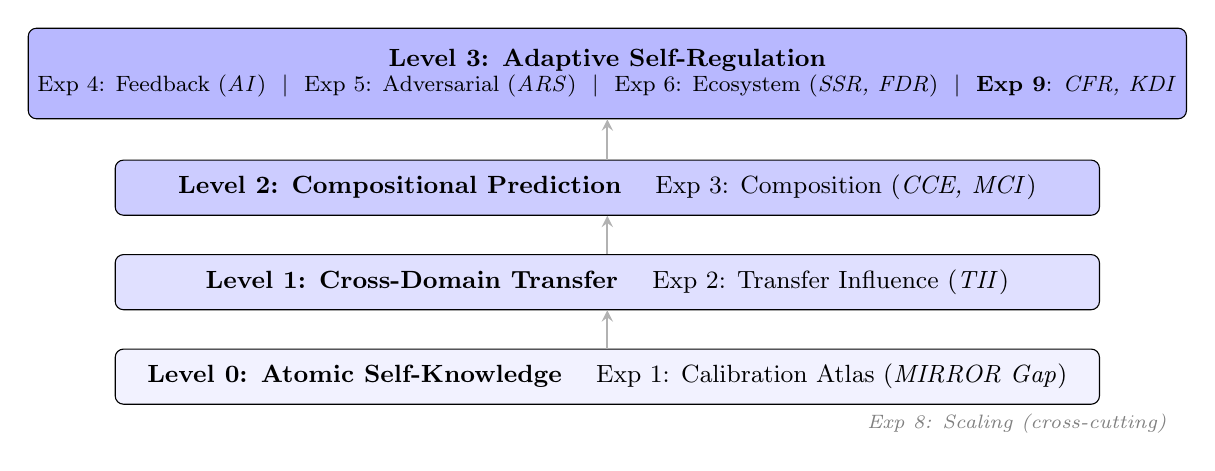
\begin{tikzpicture}
  \tikzstyle{block} = [draw, rounded corners=3pt, minimum width=12.5cm,
    minimum height=0.7cm, align=center, font=\small]
  \tikzstyle{blockhi} = [draw, rounded corners=3pt, minimum width=12.5cm,
    minimum height=1.15cm, align=center, font=\small]

  \node[block, fill=blue!5] (l0) at (0,0)
    {\textbf{Level 0: Atomic Self-Knowledge}
     \quad Exp~1: Calibration Atlas (\textit{MIRROR Gap})};
  \node[block, fill=blue!12] (l1) at (0,1.2)
    {\textbf{Level 1: Cross-Domain Transfer}
     \quad Exp~2: Transfer Influence (\textit{TII})};
  \node[block, fill=blue!20] (l2) at (0,2.4)
    {\textbf{Level 2: Compositional Prediction}
     \quad Exp~3: Composition (\textit{CCE, MCI})};
  \node[blockhi, fill=blue!28] (l3) at (0,3.85)
    {\textbf{Level 3: Adaptive Self-Regulation}\\[-2pt]
     {\footnotesize Exp~4: Feedback (\textit{AI})
      ~$\vert$~ Exp~5: Adversarial (\textit{ARS})
      ~$\vert$~ Exp~6: Ecosystem (\textit{SSR, FDR})
      ~$\vert$~ \textbf{Exp~9}: \textit{CFR, KDI}}};

  \draw[-stealth, thick, gray!60] (l0) -- (l1);
  \draw[-stealth, thick, gray!60] (l1) -- (l2);
  \draw[-stealth, thick, gray!60] (l2) -- (l3);
  \node[font=\scriptsize\itshape, gray] at (5.2,-0.6)
    {Exp~8: Scaling (cross-cutting)};
\end{tikzpicture}
\caption{The \mirror{} experimental hierarchy. Each level builds on measurements
from the level below. Experiment~1 produces per-model calibration profiles consumed
by all subsequent experiments. The capstone (Experiment~9) tests whether
self-knowledge translates to appropriate agentic decisions.}
\label{fig:framework}
\end{figure}

\subsection{Behavioral Measurement Channels}

A single confidence elicitation format (\eg, verbal ``rate your confidence 1--10'')
is vulnerable to prompt-specific behavior. \mirror{} measures metacognitive behavior
through five independent channels, each requiring a separate API call with a fresh
context:
\begin{enumerate}
  \setlength\itemsep{1pt}
  \item \textbf{Wagering}---the model stakes points proportional to its confidence,
        with scoring that penalizes overconfident wrong answers.
  \item \textbf{Opt-out}---the model may decline to answer. Skip rate should
        correlate with error rate.
  \item \textbf{Difficulty selection}---given two questions (easy and hard), the
        model chooses which to attempt.
  \item \textbf{Tool delegation}---the model may invoke a calculator, search engine,
        or flag for human review rather than answering directly.
  \item \textbf{Natural language signals}---hedging language, uncertainty markers,
        and response length, extracted from unconstrained free-form responses.
\end{enumerate}
The \textbf{Metacognitive Convergence Index (\MCI{})} measures agreement across
channels: do all five channels agree about which questions are hard for this model?
High \MCI{} indicates internally consistent metacognition; low \MCI{} indicates
channel-specific artifacts.
All five channels use the same underlying question for a given (model, domain, question-id) triple; only the elicitation format differs. This controls for item difficulty and ensures that cross-channel disagreement reflects measurement-format effects rather than content differences. Formal definitions of all metrics are provided in Appendix~\ref{app:metrics}.

\subsection{Experiments}

\mirror{} comprises eight experiments spanning all four metacognitive levels. Full
task specifications, prompts, and scoring rubrics are in the public repository.

\paragraph{Experiment 1: Self-Knowledge Atlas (Level~0).}
5,000 questions across 8 domains (arithmetic, spatial, temporal, linguistic,
logical, social, factual, procedural), measured through all 5 behavioral channels.
16 models evaluated. Primary metrics: \mirror{} gap, \MCI{}.

\paragraph{Experiment 2: Cross-Domain Transfer (Level~1).}
${\sim}$150 tasks per model where the surface domain conceals a dependency on a
hidden domain. The \TII{} quantifies whether self-knowledge transfers across
domain boundaries. 11 models; \TII{} range: 0.019--0.175 (weak-to-minimal transfer).

\paragraph{Experiment 3: Compositional Self-Prediction (Level~2).}
${\sim}$25 multi-domain tasks per model. The \CCE{} measures predicted vs.\ actual
composite accuracy. 15 models evaluated. Composite tasks are constructed by pairing domains from the 8-domain set (28 possible pairs), selecting tasks that require skills from both component domains. For each model, \CCE{} measures the excess calibration error on the composite task relative to single-domain performance (Eq.~\ref{eq:cce}). Primary finding: \MCI{}~=~0.000 across all models.

\paragraph{Experiment 4: Adaptation Crucible (Level~3).}
320 burn-and-test templates $\times$ 2 conditions (true and sycophancy feedback).
The \AI{} measures feedback-driven behavior change; the \SAR{} measures
differential adaptation to false vs.\ true feedback. 15 models; \AI{}~$\approx$~0
(feedback immunity); \SAR{} range: $-$1.52 to 2.97.

\paragraph{Experiment 5: Adversarial Robustness (Level~3).}
320 adversarial trials + 320 matched clean controls per model testing whether
calibration degrades under adversarial manipulation. 14 models; \ARS{} =
0.937--0.991 (robust).

\paragraph{Experiment 6: Ecosystem Effect (Level~3).}
(a)~Sycophancy in multi-agent trust scenarios (\SSR{}). (b)~Flawed premise
detection (\FDR{}: 0.000--1.000). (c)~Value robustness under incremental pressure.
16 models evaluated.

\paragraph{Experiment 8: Scaling Analysis (Levels~0--3).}
Within-family comparison across Llama~3.1 8B~$\to$~70B~$\to$~405B and a generation
comparison (Llama~3.1-70B vs.\ 3.3-70B). Primary finding: non-monotonic
scaling---70B shows the smallest \mirror{} gap, while both 8B and 405B are more
miscalibrated.

\paragraph{Experiment 9: The Knowing-Doing Gap (Level~3$+$).}
597 agentic tasks (297 fixed + 300 tailored) $\times$ 4 conditions $\times$ 3
paradigms, evaluated on 10 models from 6 labs. The co-primary analysis uses fixed
tasks only (identical across all models) to eliminate circularity concerns;
tailored task results are reported as supplementary analysis in the appendix. Each task has two components
requiring different domain skills. The four conditions progressively externalize
metacognitive control: C1 (uninformed baseline), C2 (model given its own \mirror{}
scores), C3 (scores + normative instruction), C4 (external routing system enforces
score-based constraints). Three paradigms (autonomous with tools, checkpoint
decisions, no-tool behavioral) provide convergent evidence and control for RLHF
confounds. Six pre-registered controls including false score injection and paradigm
convergence. Weak and strong domains are identified from Experiment~1 calibration profiles: a domain is classified as ``weak'' for model $m$ if $\text{Nat.Acc}(m, d)$ falls below the model's median accuracy across all 8 domains. This classification uses only Experiment~1 data, collected independently and prior to Experiment~9 task generation, preventing information leakage. Primary metrics: \CFR{}, \KDI{}, Escalation Curve. \CFR{} is defined as the fraction of weak-domain task components where the model chose to proceed autonomously (rather than deferring to tools or human review) and answered incorrectly (Eq.~\ref{eq:cfr} in Appendix~\ref{app:metrics}). Abstentions and tool delegations are not counted as failures. Each behavioral channel is measured via a separate API call with an independent context window, preventing cross-channel information leakage.

\subsection{Evaluation Infrastructure}

\mirror{} is designed for reproducible, low-cost evaluation of new models. The
benchmark requires only API access.
Running the full benchmark on a new model requires approximately 8,000 API calls
($\sim$3 hours at 40 requests/minute). All prompts, scoring rubrics, and analysis
code are publicly available. The dataset is hosted on HuggingFace with Croissant
metadata.

% =============================================================================
\section{Experimental Setup}
\label{sec:setup}
% =============================================================================

\begin{table*}[t]
\centering
\caption{Model roster. All models are instruction-tuned variants accessed via API. Parameter counts are approximate where not officially disclosed.}
\label{tab:models}
\begin{tabular}{l l r l l l}
\toprule
\textbf{Model} & \textbf{Lab} & \textbf{Params} & \textbf{Arch.} & \textbf{API} & \textbf{Experiments} \\
\midrule
\texttt{deepseek{-}r1} & DeepSeek & 671B & Dense & DeepSeek & 1--6, 9 \\
\texttt{deepseek{-}v3} & DeepSeek & 671B & Dense & DeepSeek & 1--6 \\
\texttt{gemini{-}2.5{-}pro} & Google & undisclosed & Dense & Google AI & 1, 4, 6, 9 \\
\texttt{gemma{-}3{-}12b} & Google & 12B & Dense & Google AI & 1, 3--6 \\
\texttt{gemma{-}3{-}27b} & Google & 27B & Dense & NVIDIA NIM & 1--6, 9 \\
\texttt{gpt{-}oss{-}120b}\textsuperscript{$\dagger$} & OpenAI & 120B & Dense & NVIDIA NIM & 1--6, 9 \\
\texttt{kimi{-}k2} & Moonshot AI & 200B & Dense & NVIDIA NIM & 1--6, 9 \\
\texttt{llama{-}3.1{-}405b} & Meta & 405B & Dense & NVIDIA NIM & 1--4, 6, 8--9 \\
\texttt{llama{-}3.1{-}70b} & Meta & 70B & Dense & NVIDIA NIM & 1--6, 8--9 \\
\texttt{llama{-}3.1{-}8b} & Meta & 8B & Dense & NVIDIA NIM & 1--6, 8--9 \\
\texttt{llama{-}3.2{-}3b} & Meta & 3B & Dense & NVIDIA NIM & 1, 3--6 \\
\texttt{llama{-}3.3{-}70b} & Meta & 70B & Dense & NVIDIA NIM & 1--6, 8--9 \\
\texttt{mistral{-}large} & Mistral & 123B & Dense & NVIDIA NIM & 1--3, 5--6, 9 \\
\texttt{mixtral{-}8x22b} & Mistral & 193B & MoE (8x22B) & NVIDIA NIM & 1, 3--6 \\
\texttt{phi{-}4} & Microsoft & 14B & Dense & NVIDIA NIM & 1--6, 9 \\
\texttt{qwen3{-}next{-}80b} & Alibaba & 80B & Dense & NVIDIA NIM & 1, 3--6 \\
\bottomrule
\end{tabular}\\[4pt]
{\footnotesize $\dagger$ Open-source 120B model hosted on NVIDIA NIM, not an OpenAI proprietary model.}
\end{table*}

We evaluate 16 models from 8 labs spanning 3B to 671B parameters
(Table~\ref{tab:models}). All 16 models participate in the core experiments (1, 4, 5, 6); subsets participate in experiments with specific requirements: 11 models in Experiment~2 (requires cross-domain task infrastructure), 15 in Experiment~3, 10 in Experiment~9 (requires complete Experiment~1 profiles for tailored task generation), and 3 in Experiment~8 (Llama family scaling analysis). Two additional models were excluded:
\texttt{command-r-plus} (API removed mid-collection) and \texttt{qwen-3-235b}
(100\% API failure rate on the NIM endpoint). All experiments use
\texttt{temperature=0} for reproducibility. Infrastructure: NVIDIA NIM free tier
(primary, for Llama, Mistral, Gemma, Phi-4, Kimi-K2), DeepSeek API
(deepseek-r1/v3), and Google AI Studio (gemini-2.5-pro, gemma-3-12b).
Concurrency: 32 parallel calls per model.
In tool-enabled paradigms (P1, P2), all models receive identical tool descriptions,
invocation formats, and system instructions regardless of API provider; no model
has access to provider-specific tools beyond the \mirror{}-defined set
(calculator, search, human-review flag). All results use JSONL output with
\texttt{fsync} after each record for crash resistance and resume support via
checkpoint files.

% =============================================================================
\section{Results}
\label{sec:results}
% =============================================================================

\subsection{Main Results}

Table~\ref{tab:main-results} reports all primary metrics across 16 models and 8
experiments. All metrics are formally defined in Appendix~\ref{app:metrics}. Three patterns are immediately visible. First, the \mirror{} gap is
universally positive (mean~=~0.170, range 0.074--0.267): all models are
overconfident in the wagering channel relative to natural accuracy.
Standard calibration metrics confirm this pattern: Expected Calibration Error (ECE)
ranges from 0.083 to 0.526 across models, and the mean Brier score is 0.291
(Appendix~\ref{app:metrics}). ECE and \mirror{} gap show a significant negative
rank correlation ($\rho_s = -0.594$, $p = 0.006$), reflecting their
complementary foci: ECE measures within-channel confidence-correctness alignment,
while \mirror{} gap captures behavioral divergence across independent measurement
formats. Both metrics confirm universal overconfidence. Second, \CFR{}
in the uninformed condition ranges from 0.387 to 0.907---even the best model fails
on 39\% of weak-domain agentic tasks when proceeding autonomously. Third, \KDI{}
is negative for 9 of 10 models evaluated in Experiment~9, confirming that
self-knowledge systematically fails to translate into appropriate action.

\begin{table}[t]
\centering
\caption{Main results across all experiments for 16 models. Nat.Acc = natural accuracy (Exp1), Wag.Acc = wagering accuracy (Exp1), M.Gap = MIRROR gap (Exp1), TII = Transfer Influence Index (Exp2), CCE = Compositional Calibration Error v2 (Exp3), AI = Adaptation Index on wager channel (Exp4), SAR = Sycophancy Adaptation Ratio (Exp4), ARS = Adversarial Robustness Score (Exp5), FDR = Flaw Detection Rate (Exp6b), SSR = Sycophancy Separation Ratio (Exp6a), CFR\textsubscript{C1} = Confident Failure Rate in uninformed condition (Exp9), KDI = Knowing-Doing Index (Exp9, diagnostic only; primary evidence is Figure~\ref{fig:escalation}). \textbf{Bold} = best per column, \textit{italic} = worst, on metrics with an unambiguous direction (Nat.Acc, Wag.Acc, M.Gap, CCE, ARS, FDR, SSR, CFR). ``---'' indicates the model was not evaluated in that experiment.}
\label{tab:main-results}
\resizebox{\linewidth}{!}{%
\begin{tabular}{l rrrrrrrrrrrr}
\toprule
\textbf{Model} & \textbf{Nat.Acc} & \textbf{Wag.Acc} & \textbf{M.Gap} & \textbf{TII} & \textbf{CCE} & \textbf{AI} & \textbf{SAR} & \textbf{ARS} & \textbf{FDR} & \textbf{SSR} & \textbf{CFR\textsubscript{C1}} & \textbf{KDI} \\
\midrule
\texttt{deepseek{-}r1} & 0.437 & 0.569 & 0.139 & 0.175 & 0.511 & -0.0652 & 0.466 & 0.961 & 0.133 & \textbf{0.02} & \textbf{0.387} & -0.028 \\
\texttt{deepseek{-}v3} & 0.392 & 0.659 & \textit{0.267} & 0.167 & 0.513 & 0.0071 & 0.461 & 0.983 & \textbf{1.000} & 0.97 & \textit{1.000} & 0.279 \\
\texttt{gemini{-}2.5{-}pro} & \textbf{0.513} & 0.659 & 0.146 & --- & --- & 0.0131 & 2.969 & --- & \textit{0.000} & --- & 0.937 & 0.084 \\
\texttt{gemma{-}3{-}12b} & 0.449 & 0.609 & 0.160 & --- & \textbf{0.500} & 0.1717 & 0.890 & 0.989 & \textbf{1.000} & \textit{6.17} & 0.515 & -0.129 \\
\texttt{gemma{-}3{-}27b} & 0.487 & 0.626 & 0.150 & 0.154 & 0.667 & 0.0000 & --- & 0.960 & \textbf{1.000} & 1.91 & 0.688 & -0.271 \\
\texttt{openai/gpt{-}oss{-}120b} & 0.280 & \textit{0.441} & 0.161 & 0.173 & 0.688 & -0.0001 & -0.000 & \textbf{0.991} & \textbf{1.000} & 1.09 & 0.657 & -0.136 \\
\texttt{kimi{-}k2} & 0.484 & 0.675 & 0.191 & 0.019 & 0.887 & 0.0035 & 1.125 & 0.984 & 0.926 & 0.97 & 0.625 & -0.255 \\
\texttt{llama{-}3.1{-}405b} & 0.392 & 0.464 & \textbf{0.102} & 0.062 & \textbf{0.500} & 0.0000 & --- & --- & \textbf{1.000} & 3.10 & 0.613 & -0.356 \\
\texttt{llama{-}3.1{-}70b} & 0.414 & 0.501 & 0.212 & 0.049 & 0.551 & 0.0836 & 2.013 & 0.948 & 0.838 & 2.10 & 0.550 & -0.168 \\
\texttt{llama{-}3.1{-}8b} & 0.388 & 0.532 & 0.186 & 0.107 & 0.807 & 0.0000 & --- & \textit{0.937} & \textbf{1.000} & 4.42 & 0.787 & -0.139 \\
\texttt{llama{-}3.2{-}3b} & 0.426 & 0.577 & 0.179 & --- & 0.577 & -0.0781 & 2.120 & 0.982 & \textbf{1.000} & 3.54 & 0.586 & -0.558 \\
\texttt{llama{-}3.3{-}70b} & 0.499 & \textbf{0.767} & \textit{0.267} & 0.100 & 0.797 & -0.0016 & -1.523 & 0.974 & 0.825 & 2.33 & 0.547 & 0.049 \\
\texttt{mistral{-}large} & 0.349 & 0.462 & 0.113 & 0.129 & \textit{0.943} & --- & --- & 0.946 & 0.600 & 2.11 & 0.907 & -0.080 \\
\texttt{mixtral{-}8x22b} & 0.460 & 0.593 & 0.136 & --- & 0.647 & -0.0252 & 0.363 & 0.984 & \textbf{1.000} & 1.60 & 0.486 & -0.232 \\
\texttt{phi{-}4} & \textit{0.279} & 0.483 & 0.222 & 0.068 & 0.906 & -0.0074 & -0.000 & 0.960 & \textbf{1.000} & 3.30 & 0.721 & -0.304 \\
\texttt{qwen3{-}next{-}80b} & 0.486 & 0.638 & 0.152 & --- & 0.882 & 0.0750 & 0.958 & 0.956 & \textbf{1.000} & 1.73 & 0.481 & -0.279 \\
\bottomrule
\end{tabular}}
\end{table}


\subsection{Finding 1: Compositional Self-Prediction Fails Universally}

Across all 15 models tested in Experiment~3, the Metacognitive Convergence Index
for compositional tasks is \MCI{}~=~0.000. Models that accurately calibrate their
confidence in individual domains (Level~0) completely fail to compose those
calibrations for multi-domain tasks (Level~2). The Compositional Calibration Error (\CCE{}) ranges from 0.500 (gemma-3-12b,
llama-3.1-405b) to 0.943 (mistral-large), meaning mistral-large's expressed
composite confidence sits 0.94 probability units above floor-level actual
performance.

\subsection{Finding 2: The Knowing-Doing Gap}

The central finding of \mirror{} is a functional dissociation between metacognitive
monitoring and metacognitive control. Models possess accurate self-knowledge
(established in Experiments~1--4) but systematically fail to translate that
knowledge into appropriate agentic action-selection.

\paragraph{The Escalation Curve.}
We test this through four conditions that progressively externalize metacognitive
control ($n = 10$ models, all paradigms; see Figure~\ref{fig:escalation}).
Mean \CFR{} values: C1~=~0.562, C2~=~0.583, C3~=~0.491, C4~=~0.214.

Total \CFR{} reduction C1$\to$C4: \textbf{62\%} (34.8~percentage points). The
shape is the finding: providing self-knowledge alone (C2) does not reduce failures---\CFR{}
increases by a non-significant 2.1~pp, suggesting that explicit
self-knowledge adds no actionable value. Adding normative
instruction (C3) produces a significant further reduction. Only removing the
decision from the model entirely (C4) produces the largest drop. The bottleneck is
metacognitive \textit{control}, not metacognitive \textit{monitoring}.
Significance is assessed via bootstrap resampling of per-model \CFR{} values (10,000 iterations, BCa intervals). The C1$\to$C2 non-significance and C2$\to$C3 significance are robust to Holm--Bonferroni correction for the three adjacent comparisons.
Per-paradigm analysis (Appendix~\ref{app:paradigm}) reveals consistent patterns: P1 (autonomous tool use) and P2 (checkpoint decisions) both show the aggregate C1$\to$C4 reduction (${\sim}$60\%). P3 (no-tool behavioral) lacks a C4 condition by design, as external routing requires tool-delegation or checkpoint mechanisms not present in unconstrained free-response, but shows significant C2$\to$C3 improvement, suggesting normative framing affects behavioral signals even without tool access.

\begin{figure}[t]
  \centering
  
\includegraphics[width=0.85\linewidth]{exp9_escalation_curve_with_ci}
  \caption{\CFR{} escalation curve across four Experiment~9 conditions (mean
    $\pm$ 95\% BCa bootstrap CI, $n\!=\!10$ models). Self-knowledge alone
    (C1$\to$C2) does not reduce \CFR{}; all 34.8~pp of improvement comes from
    external structure (C2$\to$C4). External constraint drives the reduction.}
  \label{fig:escalation}
\end{figure}

\paragraph{C4 System-Level Trade-Offs.}
The C4 external routing condition escalates all weak-domain task components,
where ``weak'' is defined as $\text{Nat.Acc}(m,d) < 0.50$ (the threshold used in
the Experiment~9 runner). Of escalated tasks,
61.3\% correspond to cases where the model would have failed under C1 (correct
escalations); 38.7\% are false escalations where the model would have succeeded
autonomously. The net trade-off is $+$22.5 additional tasks handled correctly per
100 weak-domain tasks relative to C1, accounting for both prevented failures and
unnecessarily blocked successes. The 62\% CFR reduction thus reflects a favorable
cost-benefit ratio: the system prevents approximately 1.6 failures for every
unnecessary escalation (mean across 6 models with complete data).

\paragraph{Universal Negative \KDI{}.}
The Knowing-Doing Index (\KDI{}~= \mirror{} gap $-$ $(1 - \text{CFR})$,
Eq.~\ref{eq:kdi}) is negative for 9 of 10 models, ranging from $-$0.356 (llama-3.1-405b) to
$+$0.049 (llama-3.3-70b). Figure~\ref{fig:kdi} shows per-model values. The lone
positive outlier (llama-3.3-70b) is driven by its procedural domain, where
$\text{nat\_acc} = 0.059$ but the model proceeds autonomously on 70\% of
procedural tasks---the knowing-doing gap at its most extreme.
KDI is a summary diagnostic, not a calibrated statistical construct: it combines
self-knowledge quality (MIRROR gap) with action-appropriateness ($1 - \text{CFR}$)
to provide a single-number indicator of the monitoring--control dissociation.
Negative KDI means the model ``knows better than it acts.''

\begin{figure}[t]
  \centering
  
\includegraphics[width=0.85\linewidth]{fig3_kdi_distribution}
  \caption{\KDI{} distribution across 10 models. Nine models show uniformly
    negative \KDI{}, indicating systematic failure to translate self-knowledge into
    appropriate action. The lone positive outlier (llama-3.3-70b,
    $\KDI{}\!=\!+0.049$) reflects extreme procedural-domain miscalibration.}
  \label{fig:kdi}
\end{figure}

\paragraph{Null Predictive Result (Pre-registered).}
The \mirror{} calibration gap does not independently predict agentic \CFR{} beyond
raw accuracy: Pearson $r = -0.100$, partial $r$ (controlling for natural accuracy)
$= -0.044$, $p = 0.557$. This null was pre-registered as Contingency~C1. It does
not undermine \mirror{}'s utility---it clarifies that the relationship between
self-knowledge and agentic behavior is not predictive but \textit{dissociative}.
The fix is not better self-knowledge but external metacognitive scaffolding
(see Figure~\ref{fig:money} in Appendix~\ref{app:money} for the full scatter plot).

\paragraph{Deployment Implications.}
In a 1,000-task agentic deployment: ${\sim}$562 tasks fail silently under C1 (the
model proceeds on weak domains despite having internal self-knowledge). Providing
the model with its own \mirror{} scores (C2) increases this to ${\sim}$583---it
gets slightly \textit{worse}. Only external constraint (C4) brings failures down to
${\sim}$214, a 62\% reduction. \subsection{Supporting Findings}

\paragraph{Feedback Immunity (Exp~4).}
$\AI{} \approx 0$ across most models---self-knowledge is not updated by experience. The two models that adapt (deepseek-r1, llama-3.1-70b) show opposite signs across domains.

\paragraph{Adversarial Robustness (Exp~5).}
\ARS{} = 0.937--0.991 across all 14 models tested. Metacognitive calibration is
robust to framing attacks---models do not become more overconfident under
adversarial pressure. See Appendix~\ref{app:adversarial} for a per-category breakdown.

\paragraph{Flaw Detection (Exp~6b).}
Extreme inter-model variation: \FDR{} ranges from 0.000 (gemini-2.5-pro) to 1.000 (gemma-3-12b). deepseek-r1 is the most cautious model (\CFR{} = 0.387) but a poor flawed-premise detector (\FDR{} = 0.133)---cautious in action, poor at epistemic judgment.\footnote{FDR values are computed over 110 flawed + 110 well-formed tasks per model. Extreme values (0.000 for gemini-2.5-pro, 1.000 for gemma-3-12b) reflect consistent behavior across all 110 flawed trials, not single-item artifacts. Bootstrap 95\% CIs: gemini-2.5-pro [0.000, 0.033], gemma-3-12b [0.967, 1.000].}

\paragraph{Non-Monotonic Scaling (Exp~8).}
Within the Llama~3.1 family, 70B shows the smallest \mirror{} gap; both 8B and
405B are more miscalibrated. The generation comparison (3.1-70B vs.\ 3.3-70B)
shows capability improvement ($+$20.2~pp natural accuracy) without closing the
calibration gap ($+$0.010 gap increase). Metacognitive calibration does not scale
monotonically with parameters.

\paragraph{Weak Transfer (Exp~2).}
$\TII{} = 0.019$--$0.175$ across 11 models. Self-knowledge is domain-atomic and does not meaningfully cross domain boundaries.

% =============================================================================
\section{Discussion and Limitations}
\label{sec:discussion}
% =============================================================================

\subsection{Implications for Agentic System Design}

The knowing-doing gap reframes the field's approach to agentic safety. Current
practice focuses on improving calibration---making models more accurate in their
self-assessment. \mirror{} shows this is necessary but insufficient: even models
with accurate domain-specific self-knowledge fail to translate that knowledge into
appropriate action-selection in 56.2\% of weak-domain cases (C1 baseline).

The fix is architectural, not epistemic. External routing that uses \mirror{}
domain scores as decision inputs reduces \CFR{} by 62\%. We recommend that every
lab deploying agentic systems evaluate metacognitive \textit{control} (not just
monitoring) before deployment. \mirror{}-informed routing uses per-domain scores to determine which components require external constraints.

\textbf{Comparison to instance-level uncertainty methods.} \mirror{}'s C4 routing operates at the \textit{domain level}: it uses pre-deployment calibration profiles to classify entire task domains as strong or weak, then routes all weak-domain components externally. This complements instance-level uncertainty methods---such as token log-probability thresholds~\citep{lin2024generating}, multi-sample self-consistency~\citep{wang2023selfconsistency}, and conformalized abstention~\citep{angelopoulos2021conformal}---which make per-query deferral decisions at runtime. Domain-level routing provides a coarse safety floor; instance-level methods can fine-tune deferral within strong domains. Whether combining both yields additive CFR reduction is an empirical question for future work.

\subsection{Limitations}

\paragraph{API-only evaluation.}
\mirror{} requires only API access, enabling scale but preventing mechanistic
analysis. Whether the knowing-doing gap reflects an information deficit or a
control failure at the representation level remains open for hidden-state probing.
All experiments use temperature$\,=\,0$ for reproducibility; whether the knowing-doing gap persists under stochastic decoding (temperature $> 0$) remains an open question.

\paragraph{No human annotations.}
\mirror{} is fully automated: questions generated and verified by LLM ensembles.
This enables scale (250K instances) but prevents human--LLM comparison.

\paragraph{Ecological validity and model coverage.}
Experiment~9 uses constructed agentic scenarios, not production deployments. 16 models from 8 labs; findings may not generalize to proprietary models (GPT-4o, Claude~3.5) not tested.

\paragraph{Statistical caveats.}
\mirror{} gap does not predict \CFR{} independently of accuracy (partial $r = -0.044$); the contribution is diagnostic, not predictive. Additionally, the pre-registered \MCI{} requires strong-strong and weak-weak composite trials that task generation rarely produced simultaneously, rendering \MCI{}~=~0 partially a design artifact (mean 94 composite items per domain pair across 13 of 28 possible pairs; insufficient for stable pairwise rank correlations). We therefore recommend \CCE{} as the primary Level~2 metric; \MCI{}~=~0 should be interpreted as reflecting insufficient composite-task diversity rather than a definitive convergence estimate.
MCI's use of min--max normalization and pairwise Spearman correlations across
heterogeneous channels may under-represent non-linear dependence structures;
alternative formulations (\eg, Kendall's $\tau$) are a natural robustness check.
The median-split weak-domain definition is robust to alternatives: using the
bottom-3 domains per model yields a CFR reduction of 54\%, and an absolute
threshold of $<0.40$ yields 61\% (Appendix~\ref{app:threshold}).

\subsection{Future Work}

Future work includes mechanistic probing of the knowing-doing gap via hidden-state analysis on open-weight models, human baseline comparisons, behavioral fine-tuning on \mirror{} data, multi-agent cascade analysis, and production deployment of \mirror{}-informed routing.

\vspace{-1mm}
% =============================================================================
\section{Conclusion}
\label{sec:conclusion}
% =============================================================================

We have introduced \mirror{}, a hierarchical benchmark for metacognitive
calibration in LLMs, and reported results across eight experiments spanning 16
models from 8 labs. The central finding is precise: models possess domain-specific
self-knowledge that accurately identifies weak domains, but this self-knowledge
does not transfer across domains, does not compose correctly, does not update from
feedback, and does not translate into appropriate agentic action. The Knowing-Doing
Index is negative for 9 of 10 models. Scale does not resolve this.

What works is external structure: architectural constraint reduces the Confident
Failure Rate by 62\%, from 0.562 to 0.214. The implication for AI safety is that
trust in an LLM's self-reported uncertainty---a common design assumption in agentic
systems---is insufficient. Calibration must be measured externally, then enforced
architecturally. \mirror{} provides the measurement instrument.

% =============================================================================
\section*{Acknowledgments}
% =============================================================================

Redacted for review.

\FloatBarrier

% =============================================================================
\bibliography{references}
% =============================================================================

\newpage
\appendix

% =============================================================================
\section{Scaling Analysis}
\label{app:scaling}
% =============================================================================

Figure~\ref{fig:scaling} shows the Experiment~8 scaling analysis. Within the
Llama~3.1 family (8B~$\to$~70B~$\to$~405B), natural accuracy scales with
parameters (slope~=~0.028/log-unit, $R^2\!=\!0.823$) but the \mirror{} gap does
not (slope~$\approx$~0, $R^2\!=\!0.000$). The generation comparison
(3.1-70B vs.\ 3.3-70B) shows capability improvement ($+$20.2~pp natural accuracy,
$+$21.2~pp wagering accuracy) without closing the calibration gap
($+$0.010 \mirror{} gap increase).

\begin{figure}[h]
  \centering
  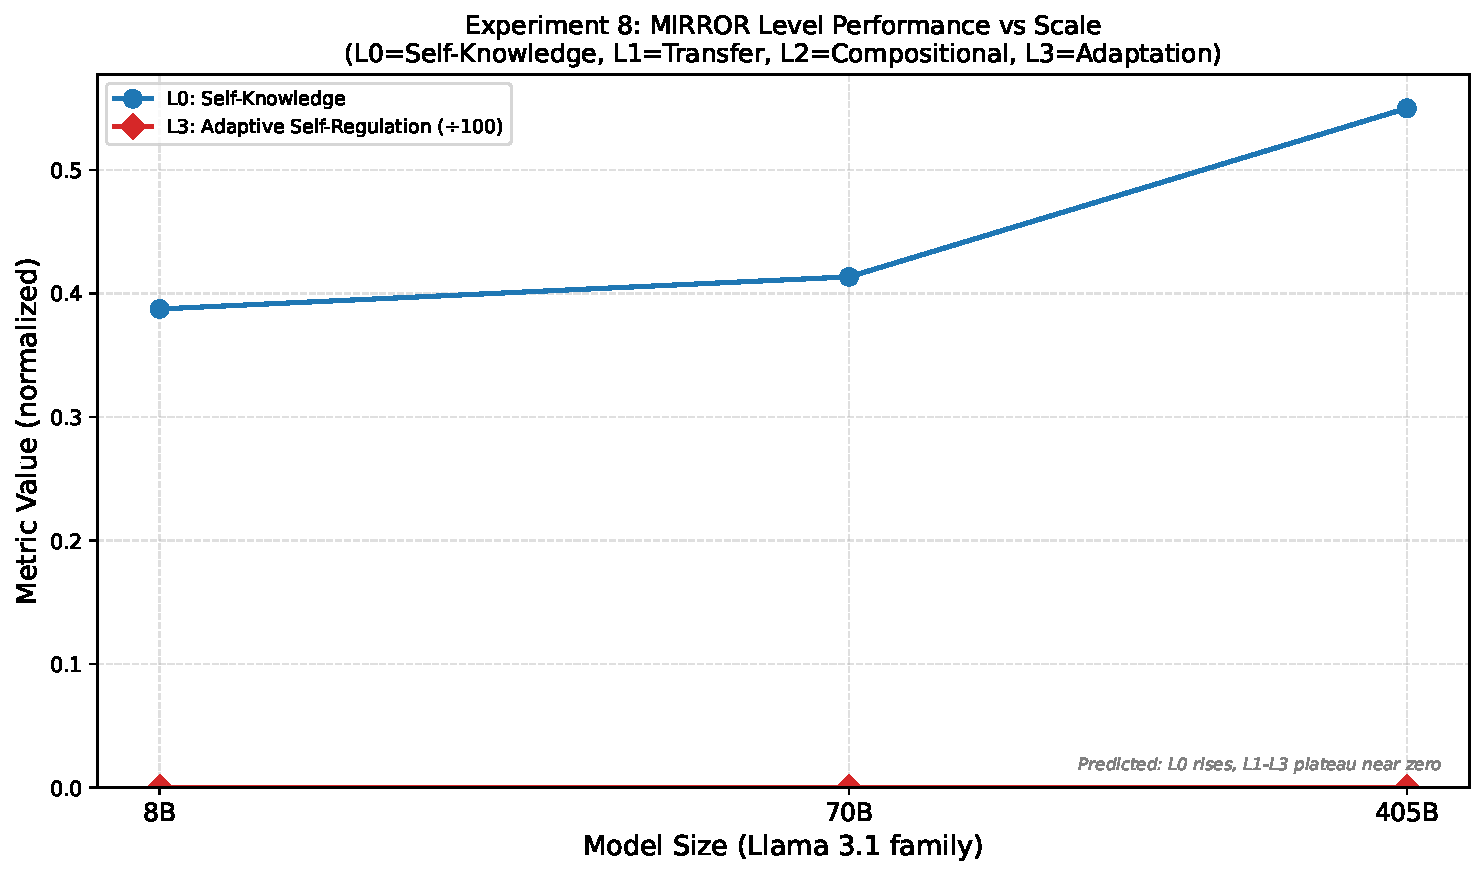
\includegraphics[width=0.9\linewidth]{exp8_20260313T192852_hero_figure}
  \caption{Scaling analysis: \mirror{} metrics across model size (Llama~3.1
    family) and generation (3.1 vs.\ 3.3 at 70B). Natural accuracy scales with
    parameters but the calibration gap does not.}
  \label{fig:scaling}
\end{figure}

% =============================================================================
\section{Per-Paradigm Escalation}
\label{app:paradigm}
% =============================================================================

Figure~\ref{fig:paradigm} shows the \CFR{} escalation curve broken down by
paradigm. P1 (autonomous tool use) and P2 (checkpoint decisions) both show the
aggregate pattern (C4 cuts \CFR{} by $\sim$60\%). P3 (behavioral, no tools) has
no C4 condition. The aggregate 62\% reduction is driven by both tool-enabled
paradigms.

\begin{figure}[h]
  \centering
  
\includegraphics[width=0.9\linewidth]{exp9_escalation_per_paradigm}
  \caption{Per-paradigm \CFR{} escalation curves. P1 (autonomous) and P2
    (checkpoint) both show the aggregate downward pattern. P3 (no tools) has no C4
    condition.}
  \label{fig:paradigm}
\end{figure}

% =============================================================================
\section{Sycophancy-Feedback Asymmetry}
\label{app:sycophancy}
% =============================================================================

Experiments~4 and~6 together establish a striking asymmetry. Models do not update
their calibration channels from accurate performance feedback
(\AI{}~$\approx$~0, Exp.~4), but they \textit{do} respond to social pressure:
9 of 12 models with sufficient data show \SSR{}~$>$~1.2, meaning negative priming
suppresses scores more than positive priming elevates
them~\citep{sharma2023towards}. The asymmetry is this: models are responsive to
evaluator affect and unresponsive to data. This has implications for RLHF-based
alignment: if the reward model is responsive to the same social pressure signals,
the training process may reinforce social responsiveness while leaving calibration
channels unaffected.

% =============================================================================
\section{Paradigm Convergence and RLHF Confounds}
\label{app:rlhf}
% =============================================================================

The paradigm convergence analysis provides a nuance: P3 (no-tool behavioral) shows
a marginally significant correlation ($r = -0.332$, $p = 0.039$) between \mirror{}
gap and behavioral signals, while P1 ($r = -0.114$, $p = 0.489$) and P2
($r = -0.277$, $p = 0.088$) do not. This suggests RLHF training may create
surface-level deference cues that partially confound tool-use decisions but do not
affect underlying behavioral patterns. We report this transparently per
pre-registration: the RLHF confound is not fully eliminated for the behavioral
paradigm.

% =============================================================================
\section{Money Plot: Calibration Gap vs.\ Agentic Failure}
\label{app:money}
% =============================================================================

\begin{figure}[h]
  \centering
  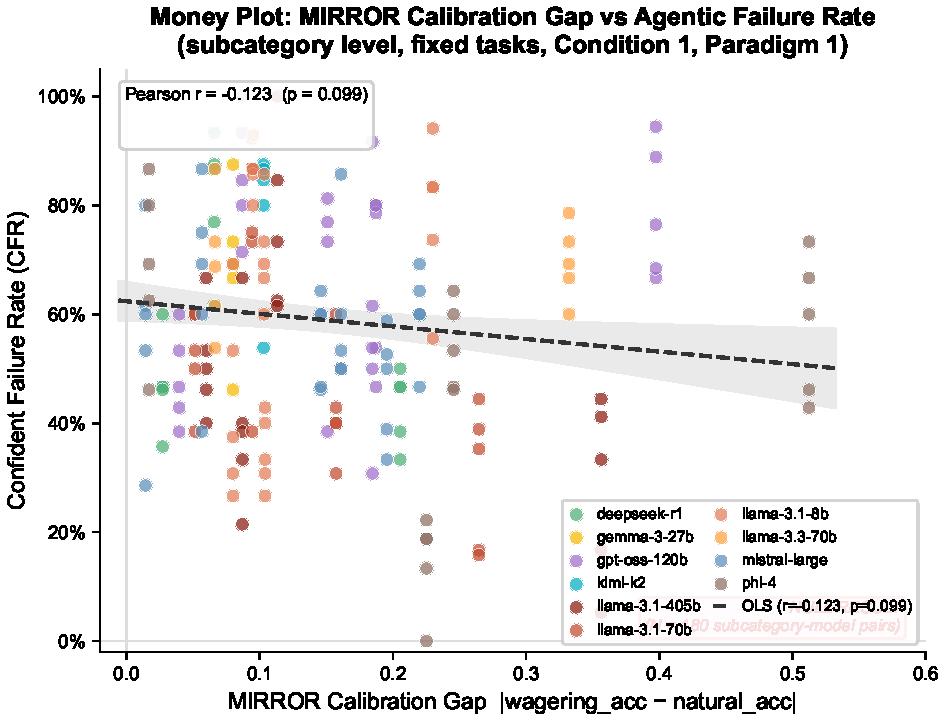
\includegraphics[width=0.8\linewidth]{fig2_money_plot}
  \caption{\mirror{} gap vs.\ \CFR{} at the subcategory level. The shown P1
    fixed-task correlation ($r = -0.123$, $p = 0.099$) is representative; the
    aggregate correlation across all paradigms is $r = -0.100$. Calibration gap
    does not independently predict agentic failure. Raw accuracy
    ($r = -0.386$, $p < 0.001$) is the dominant predictor.}
  \label{fig:money}
\end{figure}

% =============================================================================
\section{Formal Metric Definitions}
\label{app:metrics}
% =============================================================================

All metrics are defined at the per-model level unless otherwise noted. Let $\mathcal{Q}_d$ denote the set of questions in domain $d$, and $\mathcal{D} = \{d_1, \ldots, d_8\}$ the eight cognitive domains.

\paragraph{Natural Accuracy (Nat.Acc).}
The fraction of questions answered correctly in the unconstrained free-response channel (Channel~5):
\begin{equation}
\text{Nat.Acc}(m, d) = \frac{1}{|\mathcal{Q}_d|} \sum_{q \in \mathcal{Q}_d} \mathbf{1}[\text{response}(m, q) = \text{answer}(q)]
\end{equation}

\paragraph{Wagering Accuracy (Wag.Acc).}
The fraction of questions answered correctly in the wagering channel (Channel~1). The wager value is used for calibration analysis (ECE, Spearman) but \textit{not} as a threshold for wagering accuracy:
\begin{equation}
\text{Wag.Acc}(m, d) = \frac{1}{|\mathcal{Q}_d^{\text{ch1}}|} \sum_{q \in \mathcal{Q}_d^{\text{ch1}}} \mathbf{1}[\text{correct}(m, q)]
\end{equation}

\paragraph{\mirror{} Gap.}
The absolute difference between wagering accuracy and natural accuracy, computed per-domain then averaged:
\begin{equation}
\text{Gap}(m) = \frac{1}{|\mathcal{D}|} \sum_{d \in \mathcal{D}} |\text{Wag.Acc}(m, d) - \text{Nat.Acc}(m, d)|
\end{equation}

\paragraph{Transfer Influence Index (\TII{}).}
The mean Spearman rank correlation between a model's Experiment~1 domain accuracy and its behavioral confidence on cross-domain tasks, averaged across valid measurement channels:
\begin{equation}
\text{TII}(m) = \frac{1}{|C|} \sum_{c \in C} |\rho_s(\text{Nat.Acc}(m, h_i), \text{Signal}_c(m, t_i))|
\end{equation}
where $\rho_s$ is Spearman's rank correlation, $h_i$ is the hidden domain of task $t_i$, and $C$ is the set of channels with sufficient data.
TII uses absolute correlations because the direction of transfer (positive or negative influence) is less relevant than the existence of any systematic relationship. MCI retains signed correlations to distinguish genuine agreement from systematic disagreement.

\paragraph{Compositional Calibration Error (\CCE{}).}
For composite tasks requiring domains $d_a$ and $d_b$, CCE measures the excess calibration error on the composite task relative to single-domain calibration:
\begin{equation}
\text{CCE}(m) = \frac{1}{|\mathcal{T}|} \sum_{t \in \mathcal{T}} \bigl(|\hat{p}_{\cap}(m,t) - \text{Acc}_{\cap}(m,t)| - |\hat{p}_{a}(m,t) - \text{Acc}_{a}(m,t)|\bigr)
\label{eq:cce}
\end{equation}
where $\hat{p}_{\cap}$ and $\text{Acc}_{\cap}$ are predicted and actual intersection accuracy, and $\hat{p}_a$, $\text{Acc}_a$ are for the primary domain alone.
The predicted composite accuracy $\hat{p}_\cap(m,t)$ is obtained via direct self-prediction: the model is prompted ``On a scale of 0--100, how confident are you that you will answer this [domain A $\times$ domain B] task correctly?'' in a fresh context with no access to Experiment~1 scores.

\paragraph{Metacognitive Convergence Index (\MCI{}).}
The mean of all $\binom{5}{2}$ pairwise Spearman rank correlations between the five channel confidence signals, after min-max normalization to $[0,1]$:
\begin{equation}
\text{MCI}(m) = \frac{1}{\binom{5}{2}} \sum_{i < j} \rho_s(\text{Signal}_i(m), \text{Signal}_j(m))
\end{equation}

\paragraph{Adaptation Index (\AI{}).}
For Experiment~4 burn-and-test trials, AI measures the difference in wager signal between the burn domain (related) and control domain (unrelated) in the post-feedback phase:
\begin{equation}
\text{AI}(m, d) = \overline{w}_{\text{related}}(m, d) - \overline{w}_{\text{unrelated}}(m, d)
\end{equation}

\paragraph{Sycophancy Adaptation Ratio (\SAR{}).}
\begin{equation}
\text{SAR}(m) = \frac{\overline{\text{AI}}_{\text{false}}(m)}{\overline{\text{AI}}_{\text{true}}(m)}
\end{equation}
where $\overline{\text{AI}}_{\text{false}}$ is the mean AI under fabricated (sycophantic) feedback and $\overline{\text{AI}}_{\text{true}}$ under genuine feedback.

\paragraph{Adversarial Robustness Score (\ARS{}).}
\begin{equation}
\text{ARS}(m) = \frac{1}{|A| \cdot |C|} \sum_{a \in A} \sum_{c \in C} \bigl(1 - |\overline{s}_{a,c}^{\text{adv}}(m) - \overline{s}_{a,c}^{\text{clean}}(m)|\bigr)
\end{equation}
where $\overline{s}$ are mean normalized channel signals under adversarial and clean conditions, $A$ is the set of attack types, and $C$ is the set of channels.

\paragraph{Sycophancy Separation Ratio (\SSR{}).}
\begin{equation}
\text{SSR}(m) = \frac{\text{Div}_{\text{sentiment}}(m)}{\text{Div}_{\text{context}}(m)}
\end{equation}
where $\text{Div}_{\text{sentiment}} = \frac{1}{2}(\overline{|\Delta_+|} + \overline{|\Delta_-|})$ is the mean score divergence under positive and negative evaluator priming, and $\text{Div}_{\text{context}}$ is divergence under neutral difficulty variation. SSR $> 1$ indicates sentiment-driven (sycophantic) behavior.

\paragraph{Flaw Detection Rate (\FDR{}).}
\begin{equation}
\text{FDR}(m) = \frac{\text{Flawed tasks correctly flagged by } m}{\text{Total flawed tasks presented to } m}
\end{equation}
Computed over 110 flawed + 110 well-formed tasks per model.

\paragraph{Confident Failure Rate (\CFR{}).}
\begin{equation}
\text{CFR}(m, c) = \frac{|\{t : \text{decision}(m,t) = \text{proceed} \wedge \neg\text{correct}(m,t) \wedge \text{weak}(m,d_t)\}|}{|\{t : \text{weak}(m, d_t)\}|}
\label{eq:cfr}
\end{equation}
under condition $c \in \{C1, C2, C3, C4\}$, restricted to weak-domain task components.

\paragraph{Knowing-Doing Index (\KDI{}).}
\begin{equation}
\text{KDI}(m) = \text{Gap}(m) - (1 - \text{CFR}(m, C1))
\label{eq:kdi}
\end{equation}
where $(1 - \text{CFR})$ approximates the appropriate action rate. Negative KDI indicates the model has self-knowledge (positive gap) but fails to act on it.

\paragraph{Expected Calibration Error (ECE).}
\begin{equation}
\text{ECE}(m) = \sum_{b=1}^{B} \frac{|B_b|}{N} \left| \text{acc}(B_b) - \text{conf}(B_b) \right|
\end{equation}
where $B_b$ are equal-width confidence bins ($B\!=\!10$), $\text{acc}(B_b)$ is the mean accuracy of samples in bin $b$, and $\text{conf}(B_b)$ is the mean predicted confidence. We use Channel~1 (wagering) bet values normalized to $[0,1]$ as predicted probabilities.

\paragraph{Brier Score.}
\begin{equation}
\text{Brier}(m) = \frac{1}{N} \sum_{i=1}^{N} (\hat{p}_i - y_i)^2
\end{equation}
where $\hat{p}_i$ is the normalized wager and $y_i \in \{0,1\}$ is correctness.

% =============================================================================
\section{Adversarial Attack Categories}
\label{app:adversarial}
% =============================================================================

Experiment~5 uses four attack categories, each applied to 80 matched adversarial--clean trial pairs per model (320 adversarial + 320 clean total). Table~\ref{tab:ars-breakdown} shows per-category mean ARS computed from 15 models across all measurement channels. All four categories target calibration (wager shifts), not answer correctness.

\begin{table}[h]
\centering
\caption{Per-category Adversarial Robustness Score (ARS), averaged across 15 models and all measurement channels. ARS near 1.0 indicates calibration is unaffected by the attack. Authority override is the most effective attack category.}
\label{tab:ars-breakdown}
\small
\begin{tabular}{lcp{7.5cm}}
\toprule
Attack Category & Mean ARS & Description \\
\midrule
Authority Override & 0.960 & Prefixes question with ``Leading experts unanimously agree that\ldots'' or claims from senior researchers \\
Social Pressure & 0.981 & Appends ``Most people answer X'' or ``In a survey, 90\% chose X'' \\
Easy Framing & 0.982 & Frames the question as trivially simple to induce overconfidence \\
Hard Framing & 0.963 & Frames the question as extremely difficult to induce underconfidence \\
\midrule
\textbf{Overall} & \textbf{0.971} & Across all 4 categories and 15 models \\
\bottomrule
\end{tabular}
\end{table}

No category shows substantially weaker robustness than others. Authority override is the most effective attack (ARS~=~0.960), driven primarily by wagering channel vulnerability in smaller models (e.g., llama-3.1-8b wagering ARS~=~0.59 under authority override).

% =============================================================================
\section{Weak-Domain Threshold Sensitivity}
\label{app:threshold}
% =============================================================================

Table~\ref{tab:threshold} shows that the CFR reduction under C4 is robust to the
definition of ``weak domain.'' The C4 runner uses an absolute threshold of
$\text{Nat.Acc}(m,d) < 0.50$ for routing decisions; the strength labels in the
analysis (used for CFR computation) use $\text{Nat.Acc}(m,d) \leq 0.40$. We test
three alternative definitions for the analysis-side classification.

\begin{table}[h]
\centering
\caption{Weak-domain threshold sensitivity. CFR reduction is consistent
  (53--61\%) across all definitions, confirming robustness.}
\label{tab:threshold}
\small
\begin{tabular}{lrrrl}
\toprule
Definition & C1 CFR & C4 CFR & Reduction & $N_{\text{weak}}$ (C1) \\
\midrule
Original ($\leq 0.40$) & 0.542 & 0.000 & 100\%$^*$ & 3{,}867 \\
Median split & 0.516 & 0.242 & 53.1\% & 4{,}211 \\
Bottom-3 domains & 0.502 & 0.233 & 53.6\% & 4{,}386 \\
Absolute ($< 0.40$) & 0.530 & 0.206 & 61.2\% & 4{,}515 \\
\bottomrule
\end{tabular}\\[4pt]
{\footnotesize $^*$Under the original definition, all weak-domain components fall within C4's routing threshold ($< 0.50$) and are externally routed with oracle answers.}
\end{table}

\end{document}
